\chapter{Discussion and Extensions}
\label{chap:discussion}

\section{What the Implemented Connection Establishes}
The principal result is an implemented connection between a human-specified local task and an executable motion--force skill. The teaching representation supplies pose, loading, and timing together. The policy consumes observations and generates that same kind of sequence. The common executor and existing contact controller make the output actionable on the robot. E1 and E2 then examine the physical behavior rather than equating a valid network output with successful processing.

This connection is useful even though the current results do not establish a universal advantage for C. Rules and replay both achieve the required nominal loaded traversal. The exit-height reanalysis shows that the original completion-rate difference depends on recognition of the departure, while the force results favor the simpler providers in excess exposure. A task-centered interpretation therefore gives each observation its appropriate implication: a usable generated skill, functioning fixed alternatives, and an incomplete answer about robustness.

The comparison also clarifies what an execution-level result can establish. A generated rise can be learned as part of the demonstrated temporal structure. A gate can recognize unloading, and an evaluator can confirm a displacement. None of those observations directly measures remaining defect depth. Maintaining that distinction allows the method to be described positively and precisely without assigning hidden process reasoning to the policy.

\section{When Rules and Replay Are Sufficient}
The nominal task is narrow: a specified region, a single demonstrated direction, a fixed setup, and an existing lower-level controller. Under those conditions, a prescribed strategy has a strong opportunity to work well. T reuses a full force-inclusive episode and its timing, making it a substantive alternative rather than a deliberately impoverished baseline. Its short completed intervals and low observed dispersion indicate that a stable demonstration can be valuable without policy learning.

R illustrates the same point from a process-recipe perspective. A finite rule can express approach, loading, traversal, and departure directly. Its longer interval reflects the constructed strategy and contact synchronization, not an intrinsic limitation that all rules must be slower. Different recipe engineering could change that tradeoff, but no unexecuted recipe is used to reinterpret the measured comparison.

Learning becomes a stronger proposition when fixed prescriptions must respond to relevant changes in the observed task. This thesis implements a mechanism for such conditioning, but physical LOW/HIGH results are absent. The nominal comparison therefore cannot establish how much adaptation is actually supplied by that mechanism. The prepared height conditions identify a direct future test of the first research question, with the revised criterion kept distinct from the old cohort.

\section{Roles of Human Guidance and Relative Representation}
Human guidance resolves where the local operation is intended to occur. Teaching supplies an example of how movement and loading can be organized. These are complementary contributions of the operator. A spatial mask, mark, or origin cannot be treated as a complete polishing strategy, and a demonstrated strategy cannot silently substitute for a new region specification.

The relative representation supports this division by learning position around a stain center and explicitly handling the stain direction at the policy boundary. A single-direction local movement pattern is reused by aligning live XY and the policy image with the teaching direction, then inversely rotating the generated XY path and adding the live center. This is an implemented spatial-generalization mechanism, rather than a future proposal. It addresses placement and in-plane direction through task registration while leaving observation-conditioned motion--force generation to the learned policy.

Its scope follows from the transformed channels. Z, tool orientation, and force are not rotated, and image adaptation is an in-plane warp about the interaction ROI. Thus the mechanism transfers the planar movement pattern without claiming complete pose--wrench equivariance or arbitrary-view invariance. E1/E2 disable direction alignment and cannot establish its empirical rotation-transfer range. The implementation's existence and its unmeasured performance within those comparisons are separate conclusions.

The fixed image interaction ROI also has a specific function. It focuses part of the visual representation around the calibrated tool interaction area while retaining a global feature. It is not an explicit defect-state channel. The current experiments evaluate the resulting observation path as a whole; they do not isolate whether a mark's appearance, pose, or force carries most of the policy's decisions.

\section{What Force Output and Observation Contribute}
Target-force learning allows the reference sequence to express a changing load, including a departure from a constant recipe. Measured-force observation provides information about the interaction that occurred rather than the load merely requested. Their roles are conceptually distinct and are separated by the E2 contracts.

The E2 observations are consistent with differences in the organization of contact and release. A4 exposes an incomplete transition in the motion-only condition, and C has shorter operator-based intervals in this recorded cohort. However, one interrupted A attempt does not prove that missing force action caused the failure. The motion model, generated trajectory, constant-force interface, mechanical state, and timing can all contribute. Likewise, B/C are separate learned checkpoints; their difference includes the effects of separate optimization even with the same seed setting and architectural contract.

The magnitude of force peaks also limits an uncomplicated advantage claim. C does not reduce the E2 mean peak below A, and it has greater E1 excess exposure than R and T. A lower whole-window force mean can follow from less time spent in contact. It is therefore inadequate to call that lower mean an improvement in force-control accuracy or surface finishing.

The force-frame convention is another practical boundary. The resolved teaching-to-base relation supports empirical common-axis analysis, while the evaluated training file and online adapter retain their actual numerical conventions. The force-conditioning path was not redefined for this thesis. Its present performance is an observation about that implementation; a future frame-consistent learning comparison would be a separate experiment. Similarly, the executor suppresses tangential force commands, so a nine-dimensional learned action should not be described as a physically demonstrated three-axis force-tracking capability.

\section{Procedural Completion and Surface Quality}
The contact procedure is a meaningful intermediate target for local polishing. A tool must establish contact, move through the relevant region under load, and leave the surface. E1 provides explicit observations for that sequence. E2 contributes an operator-based interpretation of task progression that preserves the interrupted attempt.

Surface quality adds a separate requirement. A completed traversal may remove too little, too much, or unevenly depending on the material, tool, abrasive, speed, and pressure distribution. Visible marks may respond differently from fine scratches in metal. Before/after snapshots with changing viewpoint and occlusion cannot supply calibrated depth or roughness. Consequently, the thesis's measured results concern local contact-task execution, with visible marking changes used qualitatively.

This separation does not make the application incidental. It identifies the part of a polishing workflow that the present system actually transfers: a spatially registered temporal skill and its execution through contact feedback. It also identifies what must be added before a process-quality claim becomes defensible. The missing quality evidence cannot be replaced by a model-derived heatmap or by lower force peaks alone.

\section{Execution-Derived Dose}
\label{chap:removal_estimation}
The repository includes an execution-derived heatmap recorder. It integrates a Preston-style force--speed product along the measured path and optionally spreads it over a nominal tool kernel. Its diagnostic quantity can be expressed as
\begin{equation}
 D(x,y)=\sum_k\kappa\,F_{n,k}\,v_k\,\Delta t_k\,
                 K_{\mathrm{tool}}(x-x_k,y-y_k),
 \label{eq:preston_spatial}
\end{equation}
where \((x_k,y_k)\) is the recorded path location, \(F_{n,k}\) the implementation's selected force component or projection, \(v_k\) its selected speed, \(\Delta t_k\) the observation duration, and \(K_{\mathrm{tool}}\) a spatial spreading kernel. Without a measured coefficient and tool-response calibration, \(\kappa\) defines relative scale and \(D\) has arbitrary units. Different recorder/extension versions also make different kernel and speed-model choices.

\begin{figure}[tbp]\centering
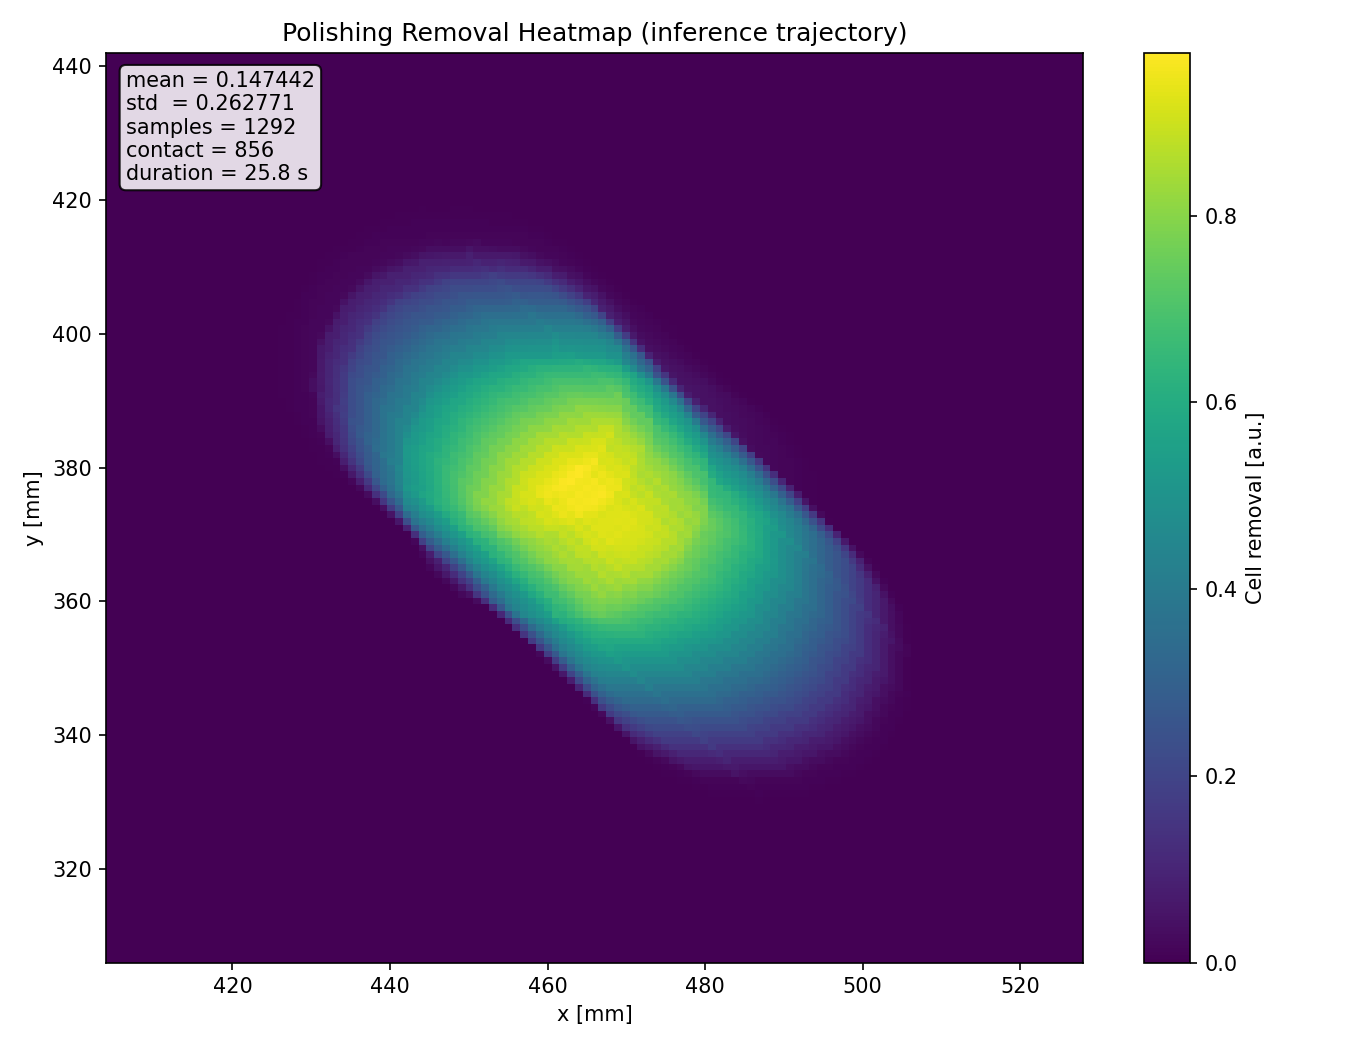
\includegraphics[width=\linewidth]{figures/E1_C1_diagnostic_heatmap.png}
\caption[Uncalibrated execution heatmap]{Existing execution-derived heatmap from E1 C1, reproduced with its original axes and colorbar. Values are an uncalibrated model diagnostic in arbitrary units. They are not measured removal depth, effective contact footprint, or surface-quality improvement. This figure is outside the primary E1 success measure.}
\label{fig:diagnostic_heatmap}
\end{figure}

The implementation and generated artifact support calling this an implemented diagnostic extension. They do not support the older claim of a calibrated material-removal model. Its spatial distribution may help inspect where modeled processing exposure accumulated, but equal dose is not demonstrated equal removal on the actual specimen.

\section{Blending and Adaptive Execution Assets}
\label{chap:blending}
The project also contains finite local blending-path generation from an existing dose map, construction of an additional spatial target, and time allocation along a path. The 13 October extension prepares a sequence in which an initial skill is followed by a separate blending pass and diagnostic displays. Its archived validation includes offline planning from an earlier execution. That is evidence of an implemented extension, not an E1/E2 surface-uniformity result.

Separate 14 October adaptive-velocity records provide development experience with reference-clock progression and replanning. The located runtime files contain five online-OFF development attempts across multiple versions. Their completion status does not establish a controlled adaptive ON/OFF process-quality comparison. A later source revision addresses a recorded stalled reference-clock case, but its README explicitly distinguishes offline checking from a new physical run. These records are therefore kept outside the nominal E2 A/B/C cohort.

\begin{table}[tbp]\centering\small
\caption[Status of inherited extensions]{Status of inherited extensions relative to the main thesis evidence.}
\label{tab:extension_status}
\begin{tabularx}{\textwidth}{P{0.32\textwidth}X}
\toprule Asset & Supported status \\ \midrule
Execution heatmap & Implemented and generated from runs; uncalibrated arbitrary-unit diagnostic. \\
Finite blending planner & Implemented; archived offline planning and integration preparation. Surface-quality improvement not established by the main comparisons. \\
Adaptive reference-clock execution & Separate versioned development attempts and code; controlled ON/OFF outcome benefit not established. \\
High-level residual RL for curved-surface restoration & Planned extension; completed skill-level training and quality-grounded evaluation not established in the selected evidence. \\
\bottomrule
\end{tabularx}
\end{table}

An earlier thesis concept proposed residual adjustments to orientation and feed velocity based on residual removal demand. That concept remains a possible extension, with its old formulation retained in the preserved source. Existing low-level learned mass/damping control is a different asset and does not validate that proposed high-level policy. The core motion--force skill in this thesis does not require a removal estimator, blending planner, or residual RL stage to count as an executable system.

\section{Limitations and Next Empirical Steps}
The immediate empirical limit is breadth. The nominal task and one trained seed per condition support a bounded comparison. Quantifying the implemented direction-transfer mechanism requires separately identified registration angles, active transfer settings, and task outcomes; E1/E2 supply no such comparison. Physical height changes, new shapes, operators, and tooling changes also require separately identified data. The prepared height protocol is the closest continuation of RQ1 because it tests an already stated research question without treating software preparation as a result.

Evaluation recognition also matters. The height-only replay demonstrates sensitivity to the initial reference, while the revised observer requires new receipt-event evidence. Future records should retain the evaluator version and observation support so that a physical strategy and its recognition can be assessed separately. Outcome corrections should remain additional interpretation records, as for A4, rather than edits to the original events.

Process-quality validation requires independent surface measurements with material and tooling records. Force-tracking validation instead requires synchronized controller-applied targets in a common frame. Neither measurement can be replaced by procedural completion.
